\documentclass[10pt,conference]{IEEEtran}
\usepackage{amsmath}
\usepackage{amssymb}
\usepackage{graphicx}
\usepackage{booktabs}
\usepackage{hyperref}

\begin{document}

\title{CAST: Testing the Attribution Stability of AI-Generated-Code Detectors Under Controlled Source Transformations}

% Double-anonymous submission: author block intentionally omitted.
\author{\IEEEauthorblockN{Anonymous Author(s)}
\IEEEauthorblockA{Submission to ICSE 2027 NIER Track}}

\maketitle

\begin{abstract}
AI-generated-code detectors are evaluated almost exclusively on static snapshots, even though real code is routinely reformatted, renamed, and restructured after creation. We present CAST (Code Attribution Stability Testing), a controlled, distance-instrumented methodology that measures whether a detector's human-versus-AI attribution survives such changes, and uses a canonicalization intervention to diagnose the source of any instability. Evaluating three independently reproducible detectors on 199 held-out Python and Java programs from the Droid corpus, we find qualitatively different stability profiles under identical transformations: DroidDetect-Base misclassifies 34.9\% of previously correct Python samples and 24.1\% of Java samples after reformatting alone, versus LLMSniffer's stable behavior and DetectCodeGPT's diffuse, family-independent instability. Canonicalizing away presentation differences attenuates DroidDetect-Base's formatting-induced instability by 14.8--63.3$\times$ but leaves DetectCodeGPT's instability essentially unchanged, showing the two failure modes have different causes. Static accuracy alone therefore does not characterize detector reliability under routine code evolution.
\end{abstract}

\begin{IEEEkeywords}
AI-generated code detection, robustness testing, metamorphic-style evaluation, software evolution
\end{IEEEkeywords}

\section{Introduction}

AI coding assistants now write a substantial share of the code developers review, edit, and ship. Detectors that attribute this code to a human or AI origin are typically evaluated the same way a classifier is: on a fixed test set, scored once, with accuracy as the verdict.

\textbf{Motivation:} That protocol quietly assumes the code being judged stays put. It does not. An IDE reformats a file on save, a refactor renames a variable, a reviewer rewrites a loop -- none of it changes what the program does, yet any of it can change what a detector says about who wrote it. A detector whose verdict flips under a cosmetic edit is not measuring origin; it is measuring the snapshot. No prior work we found treats this as something to measure directly: robustness studies vary how code is generated~\cite{hidinginplainsight}, not how it changes afterward, and detector papers report a robustness number for one perturbation at most, never a stratified account of which edits matter and why.

\textbf{Objective:} This paper's objective is to make attribution stability an explicit, measurable property of an AI-code detector, not an afterthought to accuracy, and to build the smallest instrument that can measure it. We introduce \textbf{CAST} (Code Attribution Stability Testing): given a program of known origin, CAST applies a validated transformation, measures the resulting change at the text, token, and AST level, and records how the detector's score and decision move (Section~II). Where movement is large, CAST adds a second, targeted step with no precedent in prior AI-code-detector evaluations: canonicalizing both sides of the pair to test whether the instability is a presentation artifact or something deeper. Applied to three independently reproducible detectors over 199 held-out Python and Java programs~\cite{droid}, this approach exposes stability profiles that a single accuracy number cannot: one detector's instability is almost entirely a formatting artifact that canonicalization removes; another's is not.

This paper makes three contributions.
\begin{itemize}
\item \textbf{CAST}, a controlled, distance-instrumented diagnostic methodology for evaluating attribution stability, including a canonicalization intervention with no counterpart in prior detector evaluations.
\item A held-out evaluation of three reproducible detectors over 199 programs, showing qualitatively different, transformation-specific stability profiles.
\item A canonicalization-based diagnostic distinguishing a presentation-sensitive failure mode from a broader one, together with a corpus-composition limitation that bounds this evaluation's current reach.
\end{itemize}

The remainder of the paper is organized as follows. Section~II defines CAST and the canonicalization intervention. Section~III describes the dataset, transformations, detectors, and research questions. Section~IV reports results; Section~V discusses their implications. Section~VI lists threats to validity, Section~VII positions CAST against related work, Section~VIII outlines future plans, and Section~IX concludes.

\begin{figure}[t]
\centering
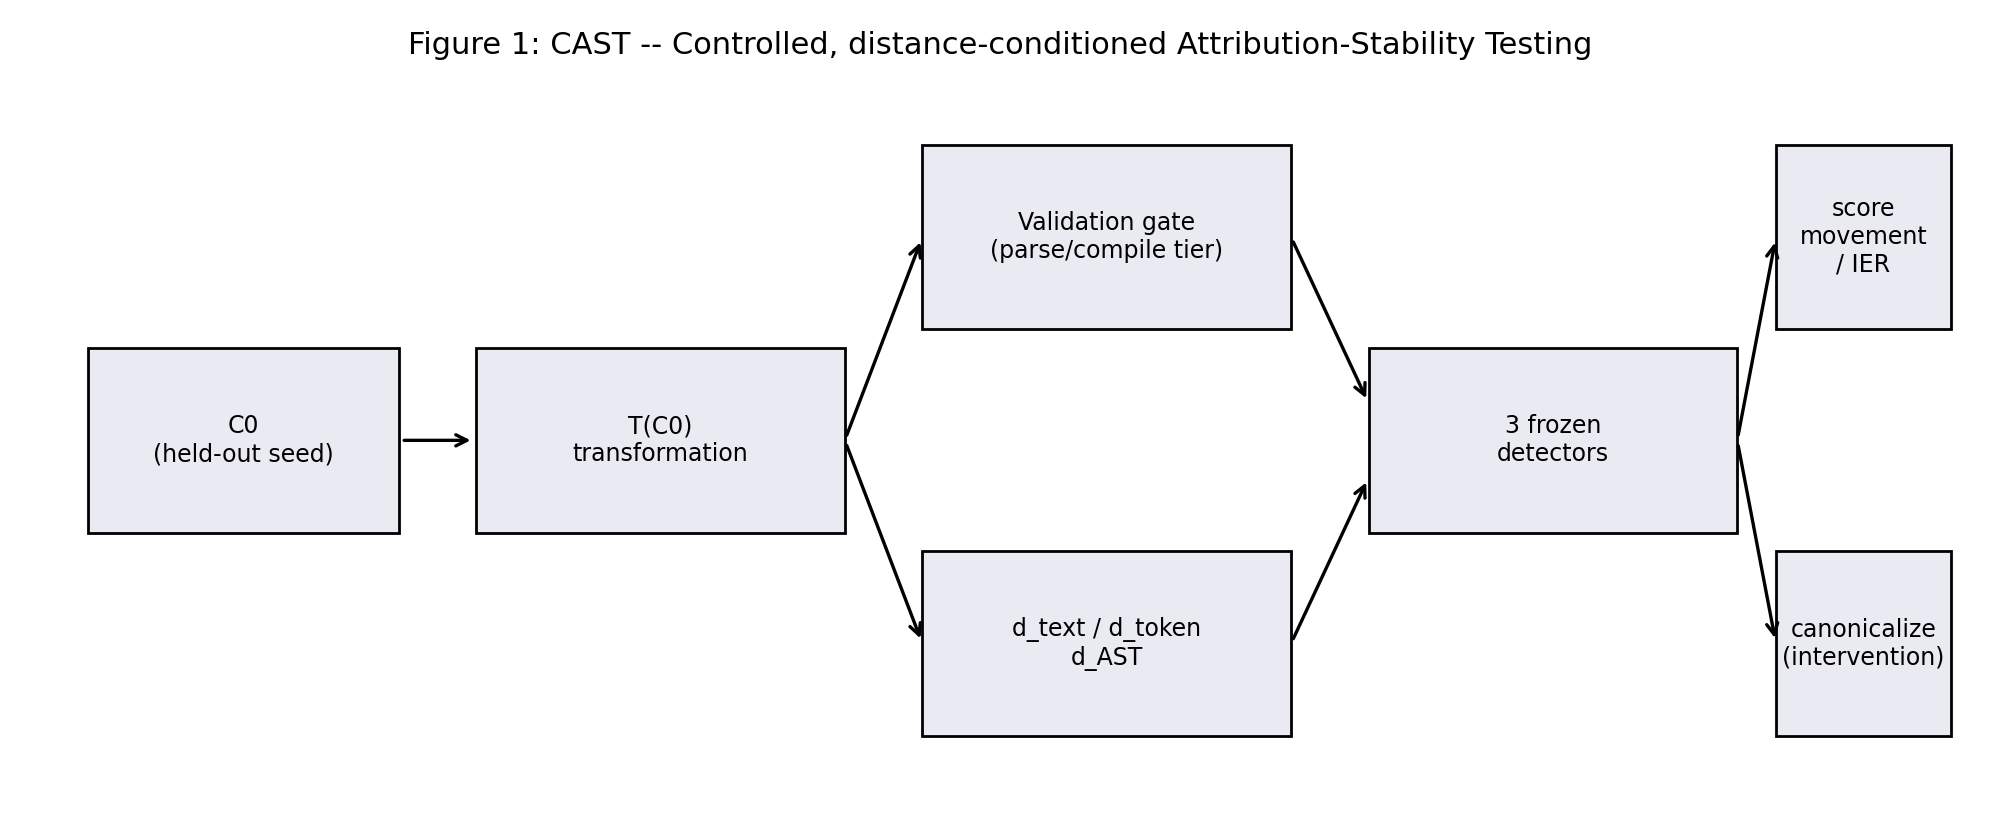
\includegraphics[width=\columnwidth]{figures/figure1_cast_methodology.png}
\caption{The CAST pipeline.}
\label{fig:cast}
\end{figure}

\section{CAST}

\subsection{Attribution stability}

\emph{Attribution stability} is the degree to which a detector's output for a program is preserved under routine, non-adversarial edits -- distinct from adversarial robustness, which studies a worst-case attacker searching for an evasive rewrite. CAST's transformations are fixed, deterministic operators applied uniformly across the corpus, not an adversarial search against any detector. CAST treats score movement and decision-flip rate as first-class observations, not a single post-transformation accuracy number.

\subsection{Methodology}

For a detector $D$, a transformation $T$, and a program $C_0$ of known provenance, CAST proceeds in five steps.
\begin{enumerate}
\item Apply $T$ to obtain $T(C_0)$.
\item Validate that $T(C_0)$ is well-formed at or above $C_0$'s own syntactic-validity tier. Non-applicable and invalid outcomes are recorded, not discarded.
\item Measure $d_\text{text}$ (character-level edit distance), $d_\text{token}$ (edit distance over the language's own lexical token stream, e.g., Python's \texttt{tokenize} output including \texttt{INDENT}/\texttt{DEDENT}, or Java tree-sitter leaves), and $d_\text{AST}$ (AST node-count change).
\item Score $D(C_0)$ and $D(T(C_0))$.
\item Aggregate, per detector, language, and family, the mean and median score movement $\Delta_D = D(T(C_0)) - D(C_0)$, the decision-flip rate, and the \textbf{Induced Error Rate}, defined as:
\end{enumerate}
\begin{equation}
\resizebox{0.99\columnwidth}{!}{$\displaystyle
\text{IER} = \frac{\#\{\text{baseline-correct programs whose decision flips after } T\}}{\#\{\text{baseline-correct programs}\}}
$}
\end{equation}
IER is conditioned on the detector having been correct on $C_0$. A flip on a program the detector already misclassified would otherwise conflate ordinary detector error with transformation-induced instability. Detectors also expose incompatible score semantics: a calibrated probability, an uncalibrated sigmoid output, or an unnormalized statistic. CAST therefore does not compare raw $|\Delta_D|$ across detectors. IER, a bounded proportion with a consistent interpretation regardless of score scale, is the primary cross-detector metric. Raw score movement is interpreted only within a given detector's own distribution.

\subsection{Canonicalization intervention}

When a transformation family produces large score movement, CAST additionally scores $F(C_0)$ and $F(T(C_0))$ for a deterministic canonicalizer $F$ that removes a specific, named category of variation (in this study: whitespace, blank lines, comments, and quote style, implemented by re-tokenizing the program and rejoining its semantic tokens). A pair for which $F(C_0){=}F(T(C_0))$ collapses to $\Delta{=}0$ by construction. This subset is reported separately from the residual pairs for which a genuine difference remains after canonicalization, so that the diagnostic result is not an artifact of the trivially-resolved cases. A substantial reduction in the residual subset's score movement constitutes intervention evidence that the removed category of variation contributes to the observed instability. It does not constitute proof of a specific internal mechanism.

\section{Study Design}

\textbf{Dataset:} This evaluation uses DroidCollection's~\cite{droid} held-out test split: 199 programs (100 Python, 99 Java), stratified across \texttt{HUMAN\_GENERATED}, \texttt{MACHINE\_GENERATED}, and \texttt{MACHINE\_REFINED}.

\textbf{Transformations:} Three confirmatory families: formatting (\texttt{black}/\texttt{google-java-format}), lexical renaming of one identifier, and control-flow rewriting (one canonical loop-form rewrite), with applicability rate 0.616 and success rate 0.992 among applicable attempts. A fourth stage attempted two deeper families, local structural extraction and semantics-preserving rewriting, reported as a feasibility finding (Section~IV-D), not a confirmatory one.

\textbf{Validation:} Python uses \texttt{compile()}-based validation. Java is tiered, given the corpus's many function/class fragments: \texttt{STANDALONE\_VALID} $>$ \texttt{WRAPPER\_VALID} (compiles inside a synthetic harness, used only as a validation instrument and never scored) $>$ \texttt{STRUCTURAL\_ONLY} $>$ \texttt{PARSE\_INVALID}.

\textbf{Detectors:} Three of five targeted detectors were independently reproducible from public artifacts. \emph{LLMSniffer}~\cite{llmsniffer} (GraphCodeBERT~\cite{graphcodebert} with a supervised-contrastive head) reaches 90.0\% sanity-check accuracy on GPTSniffer's Java test subset~\cite{gptsniffer}. \emph{DroidDetect-Base} (ModernBERT-base~\cite{modernbert} with a projection layer and a four-class head) ships a checkpoint with no modeling code; we reconstructed its architecture and validated it against a disjoint dev-split subset, reaching 87.5\% accuracy. \emph{DetectCodeGPT}~\cite{detectcodegpt} is a zero-shot statistic from the DetectGPT~\cite{detectgpt}/NPR~\cite{detectllm} family, computed from CodeLlama-7B~\cite{codellama} and CodeT5p-770M~\cite{codet5plus}, with $K{=}50$ perturbations per a pre-registered convergence study. Its threshold, calibrated on an independent 40-sample set, reaches only 60.0\% accuracy, so raw score movement is treated as primary evidence and threshold-derived decisions as secondary. \emph{GPTSniffer}~\cite{gptsniffer} and \emph{CodeGPTSensor/+}~\cite{codegptsensor} could not be integrated, as neither released a pretrained checkpoint; we did not train replacements, to avoid confounds distinct from evaluating a published detector.

\textbf{RQs:} This evaluation is structured around three research questions.
\begin{itemize}
\item \textbf{RQ1:} How stable are detector scores and decisions under formatting, lexical renaming, and control-flow rewriting?
\item \textbf{RQ2:} Do detectors exhibit similar or detector-specific stability profiles under identical transformations?
\item \textbf{RQ3:} Does canonical normalization attenuate transformation-associated instability, and does this differ across detectors?
\end{itemize}

\section{Results}

\subsection{RQ1/RQ2: detector-specific, transformation-specific profiles}

Table~\ref{tab:ier} reports IER with baseline-correct denominators. DroidDetect-Base's formatting IER is 3--12$\times$ higher than its other two families, with non-overlapping Wilson~\cite{wilson1927} 95\% confidence intervals. LLMSniffer's IER stays below 8.3\% throughout. DetectCodeGPT's IER is elevated broadly (16.7--50.0\%), peaking under control-flow rather than formatting -- diffuse, not family-localized; treated as suggestive given its calibration caveat. Median absolute score movement confirms this: DroidDetect-Base moves little except under formatting (median 0.0055, up to 0.14); LLMSniffer stays uniformly small (median 0.0106); DetectCodeGPT moves broadly regardless of family (median 0.478).

\textbf{Answer:} Stability is detector- and transformation-specific, not uniform.

\begin{table}[t]
\centering
\caption{Induced Error Rate by detector, language, and family ($n$ = baseline-correct denominator; $\dagger$ = secondary evidence).}
\label{tab:ier}
\resizebox{\columnwidth}{!}{%
\begin{tabular}{@{}llccc@{}}
\toprule
Detector & Lang. & Family & IER (n) & 95\% CI \\
\midrule
DroidDetect-Base & Py & \textbf{formatting} & \textbf{34.9\% (29/83)} & [25.6,45.7] \\
DroidDetect-Base & Java & \textbf{formatting} & \textbf{24.1\% (13/54)} & [14.6,36.9] \\
DroidDetect-Base & Py & lexical rename & 4.1\% (3/73) & [1.4,11.4] \\
DroidDetect-Base & Java & lexical rename & 2.8\% (2/71) & [0.8,9.7] \\
DroidDetect-Base & Py & control flow & 3.8\% (1/26) & [0.7,18.9] \\
DroidDetect-Base & Java & control flow & 7.1\% (1/14) & [1.3,31.5] \\
LLMSniffer & Java & formatting & 8.3\% (2/24) & [2.3,25.8] \\
LLMSniffer & Py & formatting & 6.5\% (4/62) & [2.5,15.4] \\
LLMSniffer & Py & lexical rename & 1.9\% (1/52) & [0.3,10.1] \\
LLMSniffer & Java & lexical rename & 0.0\% (0/35) & [0.0,9.9] \\
LLMSniffer & Py & control flow & 0.0\% (0/15) & [0.0,20.4] \\
LLMSniffer & Java & control flow & 0.0\% (0/4) & [0.0,49.0] \\
DetectCodeGPT$^\dagger$ & Py & control flow & 50.0\% (7/14) & [26.8,73.2] \\
DetectCodeGPT$^\dagger$ & Py & lexical rename & 30.2\% (13/43) & [18.6,45.1] \\
DetectCodeGPT$^\dagger$ & Py & formatting & 25.0\% (12/48) & [14.9,38.8] \\
DetectCodeGPT$^\dagger$ & Java & formatting & 16.7\% (6/36) & [7.9,31.9] \\
DetectCodeGPT$^\dagger$ & Java & lexical rename & 16.7\% (8/48) & [8.7,29.6] \\
DetectCodeGPT$^\dagger$ & Java & control flow & 18.2\% (2/11) & [5.1,47.7] \\
\bottomrule
\end{tabular}%
}
\end{table}

\subsection{RQ3: canonicalization intervention}

The canonicalization diagnostic was applied to all 158 formatting pairs (94 Python, 64 Java). Canonicalizing both sides collapsed \textbf{108/158 (68.4\%)} to byte-identical input ($\Delta{=}0$ by construction); the remaining \textbf{50/158} retained a residual difference and were rescored. Table~\ref{tab:canon} reports both, isolating the diagnostic's contribution from the trivially-resolved cases.

\begin{table}[t]
\centering
\caption{Mean $|\Delta|$ before/after canonicalization (not comparable across detectors).}
\label{tab:canon}
\resizebox{\columnwidth}{!}{%
\begin{tabular}{@{}lcccc@{}}
\toprule
Detector & \multicolumn{2}{c}{Full set (n=158)} & \multicolumn{2}{c}{Residual-only (n=50)} \\
 & before & after (red.) & before & after (red.) \\
\midrule
LLMSniffer & 0.026 & 0.002 (13$\times$) & 0.028 & 0.007 (3.5--3.7$\times$) \\
\textbf{DroidDetect-Base} & 0.24 & 0.006 (\textbf{40--63$\times$}) & 0.28 & 0.016 (\textbf{14.8--15.4$\times$}) \\
DetectCodeGPT & 0.67 & 0.26 (2.5--2.6$\times$) & 0.71 & 0.83 (\textbf{$\sim$1.0$\times$}) \\
\bottomrule
\end{tabular}%
}
\end{table}

On the residual-only subset -- which excludes pairs canonicalization trivially equalizes -- DroidDetect-Base's mean score movement still falls 14.8--15.4$\times$, intervention evidence that presentation variation drives most of its instability. DetectCodeGPT shows no comparable reduction, so its instability is not explained by the same presentation differences. LLMSniffer shows a smaller, real reduction on top of an already low baseline.

\begin{figure}[t]
\centering

\includegraphics[width=\columnwidth]{figures/figure3_canonicalization_intervention.png}
\caption{Canonicalization reduction factor, per detector (not cross-comparable).}
\label{fig:canon}
\end{figure}

Cohen's $d_z$~\cite{cohen1988} is reported in the accompanying artifact but not used as a headline statistic, since it standardizes by variance and can appear large even for a practically small movement (e.g., LLMSniffer, $d_z{=}1.39$--$1.49$ despite mean movement below 0.025).

\textbf{Answer:} Canonicalization explains most of DroidDetect-Base's instability but none of DetectCodeGPT's.

\subsection{Corpus feasibility for deeper transformations}

Local structural extraction and semantics-preserving rewriting were additionally attempted at two intensities. Of 796 attempted (language, family, intensity) combinations, only 37 (4.65\%) were applicable, of which 35 validated successfully. Only 4 of those 35 received true differential-execution verification. The remaining 31 degraded to structural-only validation for lack of an unambiguous, stdin-free entry point. This outcome reflects Droid's composition: a substantial share of its rows are function- or class-level fragments rather than complete executable programs, which bounds how densely this evaluation style currently extends to deeper transformations. The resulting per-detector cells ($n{=}1$--$12$) are illustrative only and support no confirmatory claim.

\section{Discussion}

Static accuracy does not characterize post-transformation reliability: all three detectors are non-trivially accurate on $C_0$, yet diverge sharply after a routine edit. The two unstable detectors' failure modes differ qualitatively, not merely in magnitude: DroidDetect-Base's instability is narrow and substantially presentation-driven, whereas DetectCodeGPT's is broad and unaffected by the same intervention. This motivates reporting stability under transformation alongside accuracy, and motivates canonicalization as a lightweight diagnostic that, for presentation-sensitive detectors, is also a candidate mitigation. CAST does not identify \emph{why} a detector is presentation-sensitive or diffusely unstable; that requires inspecting internal representations or training data, outside this paper's scope.

\section{Threats to Validity}

\begin{itemize}
\item \textbf{External:} The evaluation covers two languages, one corpus, and three reproducible detectors; two additional targeted detectors could not be integrated because no checkpoint was released. The transformation operators represent common tooling edits, not sampled developer histories.
\item \textbf{Construct:} Detector scores have incompatible scales (Section~II-B), and DetectCodeGPT's weak calibration (Section~III) limits its threshold-derived results to secondary status. $d_\text{text}$, $d_\text{token}$, and $d_\text{AST}$ are complementary but incomplete proxies for the magnitude of a program's change.
\item \textbf{Internal:} DroidDetect-Base's architecture was reconstructed from its checkpoint in the absence of public modeling code. The canonicalizer normalizes several presentation properties simultaneously, so a positive result supports a claim about that combined category of variation, not about which specific property is responsible, and does not establish an internal mechanism.
\item \textbf{Corpus:} Droid's fragment-heavy composition limits the deeper transformations to 4.65\% applicability and limits differential-execution verification to 4 of 35 successful instances. The corresponding per-detector cells are illustrative, not confirmatory.
\item \textbf{Conclusion:} Some cells have small baseline-correct denominators, as low as $n{=}4$; Wilson 95\% confidence intervals are reported throughout for this reason. Cohen's $d_z$ is treated as supplementary evidence of directional consistency only.
\end{itemize}

\section{Related Work}

Table~\ref{tab:novelty} positions CAST against the closest prior work on five dimensions: post-generation variation (Post-gen.), distance instrumentation, IER, cross-detector comparison, and canonicalization (Canon.). Detector papers~\cite{gptsniffer,llmsniffer,detectcodegpt,codegptsensor} report accuracy, occasionally under one perturbation, but none stratifies transformations or instruments distance. Pordanesh et al.~\cite{hidinginplainsight} vary training-set and prompting conditions, not the source code itself after generation. RoPGen~\cite{ropgen} applies style transformation \emph{during training} to harden a \emph{human}-authorship attributor; CAST applies controlled transformation \emph{at evaluation time} to \emph{already-trained}, unmodified AI-versus-human detectors. Feature-based work on whitespace as a detection signal~\cite{whitespaces} helps motivate the finding that formatting sensitivity can be presentation-driven.

\begin{table}[t]
\centering
\caption{Novelty positioning against the closest prior work.}
\label{tab:novelty}
\resizebox{\columnwidth}{!}{%
\begin{tabular}{@{}lccccc@{}}
\toprule
Work & Post-gen. & Distance & IER & Cross-det. & Canon. \\
\midrule
Detector papers~\cite{gptsniffer,llmsniffer,detectcodegpt,codegptsensor} & partial & -- & -- & -- & -- \\
Pordanesh et al.~\cite{hidinginplainsight} & -- & -- & -- & \checkmark & -- \\
RoPGen~\cite{ropgen} (trains detector) & \checkmark & -- & -- & -- & -- \\
\textbf{CAST (this work)} & \checkmark & \checkmark & \checkmark & \checkmark & \checkmark \\
\bottomrule
\end{tabular}%
}
\end{table}

\section{Future Plans}

This evaluation will be extended in two directions: (1) a corpus of complete, executable programs with test suites and chained, multi-step transformations, to scale beyond the 4.65\% applicability of function-level fragments (Section~IV-D) and approximate real software evolution; and (2) a detector explicitly trained against CAST's transformation families, to test whether stability can be achieved by construction rather than only diagnosed.

\section{Conclusion}

This paper presented CAST, a controlled, distance-instrumented methodology for testing attribution stability, applied to three reproducible detectors over 199 held-out Python and Java programs. The detectors show qualitatively different profiles: one shows formatting-specific sensitivity substantially attenuated by canonicalization; a second stays stable throughout; a third shows broad movement the same intervention does not attenuate. Static accuracy alone is insufficient to characterize reliability under routine code evolution.

\begin{thebibliography}{9}

\bibitem{droid} D.~Orel, I.~Paul, I.~Gurevych, P.~Nakov, ``Droid: A Resource Suite for AI-Generated Code Detection,'' \emph{EMNLP}, 2025.

\bibitem{llmsniffer} M.~L.~Dihan, A.~Muhtasim, ``LLMSniffer: Detecting LLM-Generated Code via GraphCodeBERT and Supervised Contrastive Learning,'' arXiv:2604.16058, 2026.

\bibitem{gptsniffer} P.~T.~Nguyen, J.~Di Rocco, C.~Di Sipio, R.~Rubei, D.~Di Ruscio, M.~Di Penta, ``GPTSniffer: A CodeBERT-based classifier to detect source code written by ChatGPT,'' \emph{Journal of Systems and Software}, 2024.

\bibitem{detectcodegpt} Y.~Shi, H.~Zhang, C.~Wan, X.~Gu, ``Between Lines of Code: Unraveling the Distinct Patterns of Machine and Human Programmers,'' \emph{ICSE}, 2025.

\bibitem{codegptsensor} ``Distinguishing LLM-generated from Human-written Code by Contrastive Learning,'' \emph{ACM Transactions on Software Engineering and Methodology}. Adversarially-trained variant (CodeGPTSensor+): X.~Yin, X.~Li, C.~Ni, X.~Xu, X.~Yang, ``Detecting LLM-generated Code with Subtle Modification by Adversarial Training,'' arXiv:2507.13123, 2025.

\bibitem{hidinginplainsight} S.~Pordanesh, S.~Bukhari, B.~Tan, L.~De Carli, ``Hiding in Plain Sight: On the Robustness of AI-Generated Code Detection,'' \emph{DIMVA}, 2025.

\bibitem{ropgen} Z.~Li, G.~Q.~Chen, C.~Chen, Y.~Zou, S.~Xu, ``RoPGen: Towards Robust Code Authorship Attribution via Automatic Coding Style Transformation,'' \emph{ICSE}, 2022.

\bibitem{whitespaces} S.~M.~H.~Nirob, S.~Ehsan, M.~Rahman, S.~Haque, ``Whitespaces Don't Lie: Feature-Driven and Embedding-Based Approaches for Detecting Machine-Generated Code,'' arXiv:2601.19264, 2026.

\bibitem{detectgpt} E.~Mitchell, Y.~Lee, A.~Khazatsky, C.~D.~Manning, C.~Finn, ``DetectGPT: Zero-Shot Machine-Generated Text Detection using Probability Curvature,'' arXiv:2301.11305, 2023.

\bibitem{detectllm} J.~Su, T.~Y.~Zhuo, D.~Wang, P.~Nakov, ``DetectLLM: Leveraging Log Rank Information for Zero-Shot Detection of Machine-Generated Text,'' \emph{Findings of EMNLP}, 2023.

\bibitem{codellama} B.~Rozi\`ere, J.~Gehring, F.~Gloeckle, et al., ``Code Llama: Open Foundation Models for Code,'' arXiv:2308.12950, 2023.

\bibitem{codet5plus} Y.~Wang, H.~Le, A.~D.~Gotmare, N.~D.~Q.~Bui, J.~Li, S.~C.~H.~Hoi, ``CodeT5+: Open Code Large Language Models for Code Understanding and Generation,'' arXiv:2305.07922, 2023.

\bibitem{modernbert} B.~Warner, A.~Chaffin, B.~Clavi\'e, et al., ``Smarter, Better, Faster, Longer: A Modern Bidirectional Encoder for Fast, Memory Efficient, and Long Context Finetuning and Inference,'' arXiv:2412.13663, 2024.

\bibitem{graphcodebert} D.~Guo, S.~Ren, S.~Lu, et al., ``GraphCodeBERT: Pre-training Code Representations with Data Flow,'' arXiv:2009.08366, 2020.

\bibitem{wilson1927} E.~B.~Wilson, ``Probable Inference, the Law of Succession, and Statistical Inference,'' \emph{Journal of the American Statistical Association}, vol.~22, no.~158, pp.~209--212, 1927.

\bibitem{cohen1988} J.~Cohen, \emph{Statistical Power Analysis for the Behavioral Sciences}, 2nd ed. Lawrence Erlbaum Associates, 1988.

\end{thebibliography}

\end{document}
